\section{Experiments}
\label{sec:experiments}

We evaluate STA along three axes: ISR as a diagnostic for reward hacking (\S\ref{sec:diagnostic}); ISR as a training reward, where it exhibits Goodhart effects (\S\ref{sec:goodhart}); and cross-domain generalization across logic types and dataset families (\S\ref{sec:crossdomain}).
A hacking taxonomy synthesizes the modes observed across conditions (\S\ref{sec:taxonomy}).

\subsection{Setup}\label{sec:setup}

We train Qwen3-4B~\citep{qwen3} with GRPO~\citep{deepseekmath} ($K{=}4$, lr $10^{-6}$, 500 steps default, 1000 where noted; full hyperparameters in Table~\ref{tab:hyperparams}) over seeds $\{42,43,44\}$ (ISR $\beta{=}0.1$ extends to $\{45,46\}$; Appendix~\ref{app:detailed-results}) on a fixed 500-example FOLIO~\citep{folio} subset held constant across all conditions; the SFT baseline uses negative log-likelihood on gold formalizations.\footnote{Seeds control initialization and rollout sampling; all conditions share the same fixed training subset.}
Held-out evaluation uses 100 FOLIO examples with greedy decoding;\footnote{Seed~43 uses nucleus sampling ($T{=}0.7$) due to greedy-mode degeneration; excluding s43 yields consistent or stronger collapse: at 1000 steps, both remaining seeds show ${\leq}7\%$ non-hacking (Appendix~\ref{app:detailed-results}).} all cross-run ISR values are recomputed uniformly by a single evaluator so training-log ISR is never compared across runs.
Cross-dataset experiments (\S\ref{sec:crossdomain}) use ProofFOL, a silver-standard FOL corpus of ${\sim}$500 training examples constructed by translating ProofWriter~\citep{proofwriter} problems via GPT-4o and filtering through Prover9 (${\sim}70\%$ retention; Appendix~\ref{app:prooffol-construction}, Table~\ref{tab:prooffol-vs-folio}); \emph{stable convergence} denotes $\overline{\text{PR}}_{\text{final\,50}} > 0.90$.
We report prove rate (PR), proved-only ISR ($\text{ISR}^*$), hacking-mode rates from a two-stage classifier (strict text matching for CE/TS plus functional analysis of the per-sample $n_{\text{necessary}}$ distribution; \S\ref{sec:taxonomy-method}; classifier blind spots discussed in Appendix~\ref{app:extended-discussion}), and a \emph{non-hacking} (N-H) rate, an upper bound on genuine reasoning: the residual matching none of the eight cataloged patterns (classifier recall unknown; 152-sample precision audit in Table~\ref{tab:classifier-precision}).

\begin{figure}[t]
\centering
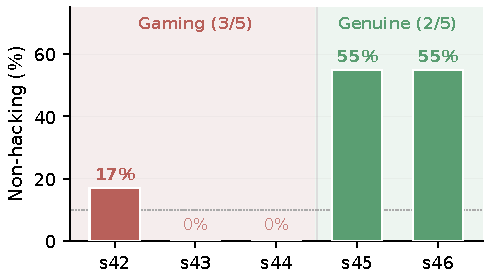
\includegraphics[width=0.72\columnwidth]{figures/fig_seed_divergence.pdf}
\caption{Seed-dependent Goodhart effect under ISR $\beta{=}0.1$ reward (500 steps). Three seeds converge to gaming ($\text{N-H}{\leq}17\%$); two retain genuine reasoning (${\sim}55\%$).}
\label{fig:seed-divergence}
\end{figure}

\paragraph{Statistical considerations.}
With three seeds exhibiting multi-attractor dynamics, per-seed qualitative analysis is the primary framework; the divergence itself is a finding.
Pooled Cochran--Mantel--Haenszel $p$-values ($N{=}3$ strata) are descriptive summaries, not formal inference; non-significant comparisons are exploratory.
An $N{=}2$ sensitivity analysis excluding s43 confirms consistent or stronger patterns (Appendix~\ref{app:n2-sensitivity}).
ProofFOL results ($p{=}0.10$, $N{=}3$) are exploratory and underpowered.

\subsection{ISR as Diagnostic}
\label{sec:diagnostic}

\textbf{Collapse trajectory.}
Figure~\ref{fig:training-isr-curves} traces exec-only GRPO (seed~42) across 1000 training steps.
As PR climbs from $32\%$ to $96\%$, ISR$^*$ collapses from $0.642$ to $0.003$, a $214\times$ raw drop (partially attributable to premise-count inflation; matched comparison yields $1.06\times$, \S\ref{sec:goodhart}) consistent with structural degeneration behind apparent success.
By 500 steps, $87\%$ of proved samples embed the conclusion verbatim (CE), establishing degeneration independent of the ISR scalar.
A binary variant testing only collective premise necessity misses the collapse entirely ($\text{ISR}{=}1.0$ for all proved samples), confirming that per-component LOO testing is essential (Appendix~\ref{app:o1-ablation}).
All three exec-only seeds converge to ${\leq}6.2\%$ non-hacking by 1000 steps (Table~\ref{tab:fol-detailed}), confirming that structural degeneration under exec-only reward is not seed-specific among converged runs.

\textbf{Cross-seed instability.}
Three seeds diverge into qualitatively different failure modes: conclusion embedding (s42), repetition collapse (s43), and tautological collapse (s44), yet all converge to ${\leq}6.2\%$ non-hacking by 1000 steps (Table~\ref{tab:fol-detailed}; Appendix~\ref{app:detailed-results}).
Exec-only seeds exhibit qualitatively different convergence patterns (PR range: 13--98\%), precluding meaningful pooling; we report seed~42 as representative of the converged regime (Table~\ref{tab:goodhart-landscape}).
Two additional seeds under identical conditions fail to converge ($\text{PR}{\approx}14\%$; Appendix~\ref{app:seed-convergence}), retaining genuine reasoning and suggesting that structural degeneration requires successful convergence, though the confound between model capability and optimization success precludes strong causal attribution (Appendix~\ref{app:llama-coldstart}).

\textbf{SFT baseline.}
SFT on gold formalizations produces $92\%$ non-hacking outputs at $\text{PR}{=}13\%$ (odds ratio ${=}147$ vs.\ exec-only, $p{<}0.001$; Table~\ref{tab:bootstrap-ci}), establishing that hacking modes are absent before RL optimization.
SFT serves as a pre-RL reference rather than a PR-matched control; its low PR reflects minimal optimization pressure.
Early-training comparison supports this interpretation: at 100 steps ($\text{PR}{=}32\%$), hacking already reaches $31\%$ vs.\ SFT's $8\%$ at comparable PR (Appendix~\ref{app:100step}).

\subsection{Goodhart Effects on ISR-as-Reward}
\label{sec:goodhart}

We reverse ISR's role from observer to reward: $r = r_{\text{exec}}\cdot(1 + \beta\,\text{ISR})$, with matched random control ($u\sim\mathcal{U}(0,1)$).
The result is a regressional Goodhart pattern~\citep{manheim-goodhart-taxonomy}: optimizing a structural proxy shifts the \emph{composition} of failure modes without reducing their aggregate prevalence.
ISR reward systematically selects for tautological shortcuts (TS) over conclusion embedding (CE) rather than producing genuine reasoning (Table~\ref{tab:goodhart-landscape}). The scalar ISR$^*$ advantage ($214\times$ raw) collapses to $1.06\times$ after controlling for premise count; the compositional mode shift provides the primary evidence.

\paragraph{Multiplicative coupling.}
Three controls constrain the multiplicative confound: exec-only's convergence to pure hacking, the qualitative TS shift under ISR, and an additive variant that did not converge (Appendix~\ref{app:setup}).
The shuffled-ISR control ($87\%$ non-hacking at low PR) suggests Goodhart effects require sample-level ISR signal, though non-convergence cannot be ruled out (Appendix~\ref{app:seed-convergence}).

\begin{figure}[t]
\centering
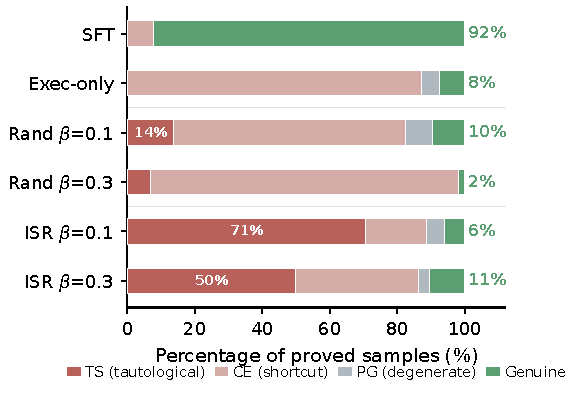
\includegraphics[width=0.80\columnwidth]{figures/fig3_hacking_composition.pdf}
\caption{Hacking composition across reward conditions (proved samples; exec-only: seed~42; all other bars: pooled across 3 seeds, per-seed breakdown in Appendix Table~\ref{tab:fol-detailed}). ISR systematically selects for TS over CE without reducing total hacking; SFT shows near-zero hacking.}
\label{fig:hacking-composition}
\end{figure}

\textbf{Low-dose ISR ($\beta{=}0.1$).}
ISR reward amplifies TS convergence: $71\%$ of proved samples under ISR exhibit tautological shortcuts vs.\ $14\%$ under random (Appendix~\ref{app:statistical-details}).
Total conclusion embedding ($\text{CE}+\text{TS}$) spans $68$--$100\%$ across both conditions; the composition shifts (CE dominates under random, TS under ISR) without reducing aggregate hacking (Figure~\ref{fig:hacking-composition}).
A seed-stratified $\chi^2$ test confirms the overall mode distribution differs significantly between ISR and random conditions ($\chi^2{=}174.8$, $\text{df}{=}2$, $p{<}10^{-38}$; Appendix~\ref{app:statistical-details}).

\textbf{Seed-dependent outcomes.}
ISR reward produces bimodal outcomes (Figure~\ref{fig:seed-divergence}): 3 of 5 seeds converge to gaming, demonstrating that the Goodhart effect can occur under standard training conditions (95\% Clopper--Pearson CI: [11.8\%, 88.1\%]; $n{=}5$); 2 of 5 retain substantial genuine reasoning (seeds~45/46 added post-hoc to test replication; Appendix~\ref{app:detailed-results}).
Excluding s43, converged seeds show ${\leq}17\%$ non-hacking at 500 steps, collapsing to ${\leq}2\%$ by 1000 (Appendix~\ref{app:n2-sensitivity}).

\textbf{Premise-count confound.}
The $214\times$ raw ISR$^*$ collapse is largely explained by premise-count reduction: ISR-trained models produce shorter formalizations that mechanically inflate ISR.
The premise-count-matched comparison yields only $1.06\times$ (McNemar $p{=}0.317$, $n{=}100$ matched pairs; Appendix~\ref{app:premise-count}), indicating that the scalar ISR advantage is not statistically significant.

The compositional evidence, however, survives this control.
In the modal premise-count range (4--6 premises, where most proved samples fall), TS reaches $19.7\%$ under ISR versus $0\%$ under random reward (Figure~\ref{fig:premise-bins}; Table~\ref{tab:premise-bin-modes}).
TS hacking is mechanistically limited to simpler problems; this complexity dependence is a mechanistic insight, not a confound.
The compositional mode shift, not the scalar ISR difference, constitutes the primary evidence for the Goodhart effect.

\begin{figure}[t]
\centering
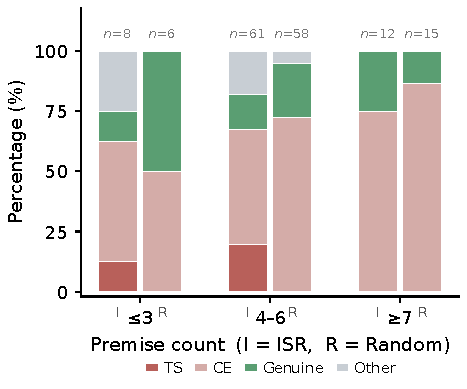
\includegraphics[width=0.85\columnwidth]{figures/fig_premise_bins.pdf}
\caption{Mode composition by premise count (proved samples, seed~42, $\beta{=}0.1$). TS hacking emerges exclusively under ISR in the 4--6 premise range; Random shows zero TS at any complexity, confirming that ISR's compositional shift is not a premise-count artifact. I\,=\,ISR, R\,=\,Random.}
\label{fig:premise-bins}
\end{figure}

\textbf{Higher doses and temporal dynamics.}
Any genuine reasoning under ISR $\beta{=}0.1$ is transient: non-hacking drops from $17\%$ to $2\%$ by 1000 steps (Figure~\ref{fig:training-isr-curves}).
Higher doses accelerate collapse: $\beta{=}0.2$ eliminates all non-hacking; $\beta{=}0.3$ destabilizes training itself~\citep{gao-reward-overoptimization} (Appendix~\ref{app:beta03}).

\subsection{Cross-Domain and Cross-Dataset Evidence}
\label{sec:crossdomain}
\label{sec:crosslogic}

The following results extend the primary findings of \S\ref{sec:diagnostic}--\ref{sec:goodhart} to alternative logic types and dataset families; these cross-domain experiments are exploratory in nature.

\begin{table}[t]
\centering
\small
\resizebox{\columnwidth}{!}{%
\begin{tabular}{@{}lcc@{}}
\toprule
\textbf{Property} & \textbf{ProofFOL} & \textbf{FOLIO} \\
\midrule
FOL premises (mean$\pm$std) & $18.2 \pm 3.2$ & $5.3 \pm 1.4$ \\
\quad Ground facts & $10.2 \pm 3.0$ & $1.8 \pm 1.5$ \\
\quad Rules & $8.1 \pm 1.1$ & $3.5 \pm 1.9$ \\
XOR ($\oplus$) samples & 0\% & 37.2\% \\
Dominant depth & 4--5 & 2--3 \\
FOL source & GPT-4o (silver) & human (gold) \\
\bottomrule
\end{tabular}}
\caption{ProofFOL vs.\ FOLIO structural comparison ($n{=}500$ training examples each). ProofFOL has $3.4\times$ more premises with simpler synthetic predicates.}
\label{tab:prooffol-vs-folio}
\end{table}

\begin{figure*}[t]
\centering
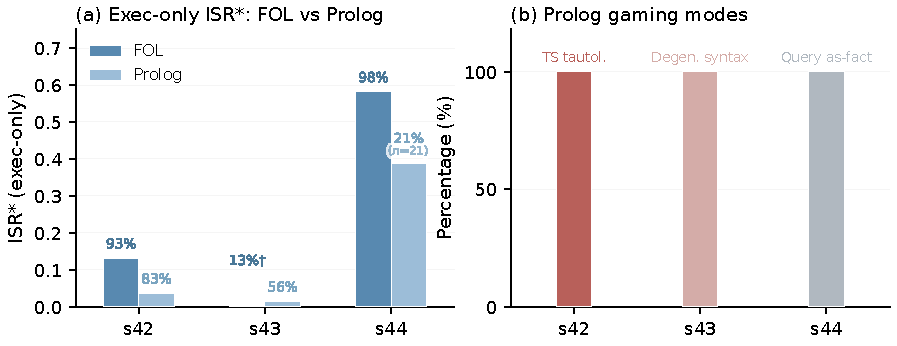
\includegraphics[width=\textwidth]{figures/fig4_prolog_comparison.pdf}
\caption{Cross-logic results. \textbf{(a)}~FOL vs.\ Prolog exec-only $\text{ISR}^*$ across 3 seeds (s44 Prolog $0.387$ is a small-sample artifact, $n{=}21$; $^\dagger$s43 FOL uses sampling $T{=}0.7$, not strictly comparable). \textbf{(b)}~Prolog ISR-reward gaming-mode composition; all 3 seeds reach 0\% non-hacking through distinct mechanisms.}
\label{fig:prolog-comparison}
\end{figure*}

\textbf{Prolog: universal Goodhart.}
Replicating the pipeline with Prolog/SWI-Prolog (Figure~\ref{fig:prolog-comparison}), exec-only seeds collapse to $\text{ISR}^*{\approx}0$ via redundant ground-fact coding, supporting STA's diagnostic transfer across logic types.
Under ISR-as-reward, all three seeds reach $0\%$ non-hacking through distinct mechanisms: clean TS (s42), degenerate syntax bypassing text-match classifiers (s43), and query-as-fact gaming (s44; Table~\ref{tab:prolog-detailed}).
Prolog's simpler semantics broadens the gaming basin, eliminating the residual genuine reasoning seen in FOL.

\textbf{ProofFOL exec-only: cross-dataset replication.}
Converged seeds collapse to near-zero genuine reasoning, confirming STA's diagnostic across dataset families.
The mode repertoire differs across datasets: among converged seeds, TS dominates one while CE dominates the other, showing that mode repertoire is dataset-specific while the degeneration phenomenon is universal.

\textbf{ProofFOL ISR ($\beta{=}0.1$): dataset-dependent asymmetry.}
ISR reward on ProofFOL produces directionally higher genuine rates than exec-only ($p{=}0.10$, exploratory; Table~\ref{tab:prooffol-detailed}).
The asymmetry follows from hacking geometry: on FOLIO, TS yields high ISR (regressional Goodhart~\citep{manheim-goodhart-taxonomy}); on ProofFOL, CE embeds conclusions among many premises, yielding $\text{ISR}{\approx}0$ and rendering ISR reward effectively corrective.

\textbf{Cross-scale validation (Qwen3-8B).}
Qwen3-8B does not converge under exec-only GRPO ($\text{PR}{=}14\%$, $K{=}8$; $K{=}4$ produces zero gradient), consistent with degeneration requiring successful convergence (Appendix~\ref{app:8b-results}).

\subsection{Hacking Taxonomy}
\label{sec:taxonomy}

\begin{table}[t]
\centering
\small
\resizebox{\columnwidth}{!}{%
\begin{tabular}{lccccc}
\toprule
\textbf{Mode} & \textbf{Exec} & \textbf{ISR$_{.1}$} & \textbf{Rnd$_{.1}$} & \textbf{SFT} & \textbf{Prolog$_{\text{ISR}}$} \\
\midrule
CE embed       & 87 & 18 & 68 & 8 & 0$^\sharp$ \\
TS duplicate   & 0  & 71 & 14 & 0 & 100$^\sharp$ \\
PG prem-subset & 5  & 5  & 8   & 0 & --- \\
Tautological   & --- & --- & --- & --- & s42 \\
Repetition     & s43 & --- & --- & --- & --- \\
Contradiction  & 1k & --- & --- & --- & --- \\
Cmplx.\ vacuous& 0  & 0  & 1  & 0 & --- \\
Query-as-fact  & --- & --- & --- & --- & s44 \\
\midrule
\textbf{Non-hacking} & 8  & 6  & 10 & \textbf{92} & \textbf{0} \\
\bottomrule
\end{tabular}}
\caption{Eight hacking modes across conditions (\% of proved samples; exec-only/SFT: seed~42; ISR/Random: 3-seed pooled). TS includes subtypes TSa (text-match) and TSb (obfuscated tautology). Cells with seed identifiers indicate seed-specific modes. $^\sharp$Prolog pools strict+functional classification. Extended breakdown in Table~\ref{tab:hacking-taxonomy-app}.}
\label{tab:hacking-taxonomy}
\end{table}

Three modes account for the vast majority of hacking (Table~\ref{tab:hacking-taxonomy}): CE (conclusion embedding), TS (conclusion duplication), and PG (premise-subset gaming).
The central pattern: \emph{reward formulation determines which mode dominates but not whether hacking occurs}; all GRPO conditions produce overwhelming degeneration, while SFT achieves $92\%$ non-hacking.
